% -*- Mode:TeX -*-

%% IMPORTANT: The official thesis specifications are available at:
%%            http://libraries.mit.edu/archives/thesis-specs/
%%
%%            Please verify your thesis' formatting and copyright
%%            assignment before submission.  If you notice any
%%            discrepancies between these templates and the 
%%            MIT Libraries' specs, please let us know
%%            by e-mailing thesis@mit.edu

%% The documentclass options along with the pagestyle can be used to generate
%% a technical report, a draft copy, or a regular thesis.  You may need to
%% re-specify the pagestyle after you \include  cover.tex.  For more
%% information, see the first few lines of mitthesis.cls. 

%\documentclass[12pt,vi,twoside]{mitthesis}
%%
%%  If you want your thesis copyright to you instead of MIT, use the
%%  ``vi'' option, as above.
%%
%\documentclass[12pt,twoside,leftblank]{mitthesis}
%%
%% If you want blank pages before new chapters to be labelled ``This
%% Page Intentionally Left Blank'', use the ``leftblank'' option, as
%% above. 

\documentclass[12pt,twoside]{mitthesis}
\usepackage{lgrind}

% Math and physics packages
\usepackage{amsmath}
\usepackage{amssymb}
\usepackage{physics}
\usepackage{upgreek}
\usepackage{xcolor}

% New commands

\newcommand{\jcp}{Journal of Chemical Physics}
\newcommand{\physrep}{Physics Reports}
\newcommand{\pra}{Physical Review A}
\newcommand{\prb}{Physical Review B} 

% For hyperlinks
\usepackage{hyperref} % For hyperlinks
\hypersetup{
 colorlinks = false, % colors links instead of ugly boxes
 urlcolor = blue, % color for external hyperlinks
 linkcolor = blue, % color for internal links
 citecolor = red % color for citations
}
\usepackage{url}
\usepackage[normalem]{ulem}
%\usepackage[hyperref=true,doi=false,url=false,isbn=false,backend=bibtex,style=nature]{biblatex}
%\usepackage{abntcite}

% For images and Figures
\usepackage{lscape}
\usepackage{graphicx}
\graphicspath{{./Images/PDFs/}} % Sets the path to the images as a subdirectory included in the same directory as the .tex file. 

%% These have been added at the request of the MIT Libraries, because
%% some PDF conversions mess up the ligatures.  -LB, 1/22/2014
\usepackage{cmap}
\usepackage[T1]{fontenc}
\pagestyle{plain}

%% This bit allows you to either specify only the files which you wish to
%% process, or `all' to process all files which you \include.
%% Krishna Sethuraman (1990).

%\typein [\files]{Enter file names to process, (chap1,chap2 ...), or `all' to
%process all files:}
\def\all{all}
\ifx\files\all \typeout{Including all files.} \else %\typeout{Including only \files.} \includeonly{\files} \fi

% Formatting
\raggedbottom

% Extra colors

%\definecolor{cerisepink}{rgb}{0.93, 0.23, 0.51}
\definecolor{navyblue}{rgb}{0.0, 0.0, 0.5}
%\definecolor{mediumelectricblue}{rgb}{0.01, 0.31, 0.59}
%\definecolor{ao(english)}{rgb}{0.0, 0.5, 0.0}
\definecolor{deepmagenta}{rgb}{0.8, 0.0, 0.8}
\definecolor{dolla-bill}{rgb}{0.52, 0.73, 0.4}

\begin{document}

\include{cover}
% Some departments (e.g. 5) require an additional signature page.  See
% signature.tex for more information and uncomment the following line if
% applicable.
% \include{signature}
\pagestyle{plain}
\include{contents}
%% This is an example first chapter.  You should put chapter/appendix that you
%% write into a separate file, and add a line \include{yourfilename} to
%% main.tex, where `yourfilename.tex' is the name of the chapter/appendix file.
%% You can process specific files by typing their names in at the 
%% \files=
%% prompt when you run the file main.tex through LaTeX.

\chapter{The Nitrogen Vacancy Center in Diamond}

\section{Introduction}

The nitrogen-vacancy (NV) defect center in diamond is currently of great interest for many applications in quantum sensing \cite{taylor2008high,balasubramanian2008nanoscale,dolde2011electric,neumann2013high, degen2008scanning,hodges2013timekeeping} and quantum information \cite{childress2013diamond,gaebel2006room,dutt2007quantum} due to its many outstanding properties, which include long room temperature coherence times \cite{balasubramanian2008nanoscale} and simplicity of optical quantum state initialization and readout \cite{schirhagl2014nitrogen,jensen2017magnetometry}. An active area of effort is NV magnetometry, with recent demonstrations of measurement modalities ranging from scanning magnetic microscopy \cite{degen2008scanning} to wide-field imaging \cite{pham2011magnetic} to bulk magnetometry \cite{wolf2015subpicotesla}. Many of these modalities address ensembles of NV centers and therefore require strong and uniform microwave (MW) field driving, often over mm length scales. In this thesis I discuss the design considerations of a suitable MW delivery mechanism, fabricate a hole-and-slot type loop gap resonator (LGR), and evaluate its performance for NV applications. 

As an introduction to the field of quantum sensing using NV centers Chapter 1 deems to introduce the photophysics of the NV\footnote{A detailed derivation of the NV level structure using group theoretic approach can be found in \cite{} }, the NVs use in continuous wave and pulsed magnetometry schemes, the importance of uniform microwave (MW) driving and previous resonant enhancement techniques, along with an introduction to the hole-and-slot type loop gap resonator featured in Chapters 2-5 and a discussion of popular coupling techniques.

Chapter 2 gives a detailed theoretical analysis of the loop gap resonator and its use in experiments utilizing electron spin resonance (ESR). It also steps through the design process of the LGR and excitation circuitry and discusses the considerations involved when choosing the device geometry and attempting to match the LGR over a wide bandwidth.

%Chapter 3 describes the LGR coupling techniques used in the experiment along with the design process of the matching circuit.

Chapter 4 discusses the MW field distribution and strength provided by the fundamental mode of the manufactured LGR using both experiment and simulations. 

Chapter 5 provides an analysis of the device's uses in NV magnetometry as well as an outlook to future of the LGR for quantum sensing.  


\section{The NV Physical and Electronic Structure} \label{sec:NVP}

%This section needs work, need to give NV Hamiltonian etc etc etc.

The negatively-charged NV color center (NV\textsuperscript{-}) is a deep band gap impurity within the diamond crystal lattice. Its inclusion in the $C_{3v}$ point group permits a $\textsuperscript{3}A_2$ symmetric spin-triplet ground state and an excited $\textsuperscript{3}E$ state separated by a zero phonon line (ZPL) of 637nm [Fig \ref{Fig_one} (a)] \cite{maze2011properties}. The ground state spin triplet is split via spin-spin interactions giving rise to a zero field splitting separating the $\ket{m_s = 0}$ from the $\ket{m_s = \pm 1}$ states by 2.87GHz (\textit{D\textsubscript{gs}}). 
The NV Hamiltonian, neglecting 


Application of a static magnetic field B\textsubscript{0} splits the $\ket{m_s = \pm1}$ levels via Zeeman interaction proportional to the projection of the field onto the NV symmetry axis. When the NV is driven into one of these states and optically excited (generally achieved using 532nm CW or pulsed laser) it undergoes phononic-relaxation and settles into the corresponding sublevel of the excited state. These sublevels allow the NV to preferentially decay back down to the $\ket{0}$ ground state via an inter-system crossing and metastable state which are separated in the infrared. This non-spin-conserving process therefore provides the mechanism of spin polarizing the NV for continued MW driving. The NV spin state can then be read out by sweeping the driving microwave field and monitoring NV fluorescence in the visible band. A drop in fluorescence at a particular driving frequency indicates electron spin resonance (ESR) which can be monitored via lock-in amplification for any detuning due to a change in the external field\cite{jensen2017magnetometry,rondin2014magnetometry}. Since the NV can exist in one of four possible orientations---each orientation being equally likely---the ESR can be separated into eight distinct non-degenerate resonances which probe different field components. The various orientations act as basis vectors which collectively span the space and allow the total vector field to be reconstructed \cite{jensen2017magnetometry}. 

\begin{figure}[t!]
\centering
\includegraphics[width =\textwidth]{Intro_Fig_1.pdf}  
\caption{\textbf{The NV center} \textbf{a)} The NV level structure \textbf{b)} One of four crystal orientations of the NV.}
\label{Fig_one}
\end{figure}

\section{Vector Magnetometry with NV Centers}\label{ch1:vect}

As mentioned in section \ref{sec:NVP}, the $C_{3v}$ symmetry of diamond allows NV centers to be aligned in four different orientations in the lattice. Since, at fields lower than 10 mT, the Zeeman splitting of the $\ket{\pm 1}$ is proportional to the vector field projection along the NV symmetry axis\footnote{At these low fields the terms in the NV Hamiltonian (see equation \ref{equ:NVHam}) that are proportional to the perpendicular component of the field are suppressed to order $\sim B_{xy}^2 / D_{gs}$ and can therefore be neglected\cite{taylor2008high}} ($B_z$) the energy shifts can be determined by $\text{g}_\text{s} \upmu \text{b}\textbf{B} \cdot \textbf{\text{u}}_n$ where $\textbf{\text{u}}_n$ ($n = 1,2,3,4$) is the unit vector along the n\textsuperscript{th} NV axis. By either sequentially or simultaneously measuring the Zeeman splitting between either the $\ket{0} \leftrightarrow \ket{+1}$ or $\ket{0} \leftrightarrow \ket{-1}$\footnote{The transition $\ket{-1} \leftrightarrow \ket{+1}$ can also be employed which yields the benefit that the energy shift becomes $2\text{g}_\text{s}\upmu_\text{b}\textbf{B}$ and therefore provides twice the signal over the other two transitions while simultaneously mitigating temperature effects \cite{neumann2013high}. However, this requires treatment of the full three-level spin system since the $\ket{-1} \leftrightarrow \ket{+1}$ splitting is a non-dipole allowed transition.} transitions of all four orientations, one can reconstruct the total vector field by generating the vector components ($B_x$, $B_y$, and $B_z$) from the projection along each of the crystallographic axes \cite{kitazawa2017vector,schloss2018simultaneous}.

\subsection{NV Ensemble Magnetic Sensitivity}



%Talk about spin projection noise, photon shot noise, minimum detectable field \delta B, SNR etc.... see Scott and Chris's thesis

%need to mention \beta, collection rate, C contrast etc here because I use it in the sections below ----- and ODMR

%Talk about using N NVs to enhance sensitivity (look up Hannah paper how they calculate)

% Talk about how sensitivity in an ensemble is increased by 1/sqrt{N} but denser packing of N reduces T_2^* and therefore broadens the minimum achievable bandwidth in an NV experiment.

% Optional: Briefly talk about other readout mechanisms like photoelectric readout, IR absorption readout etc.

\subsection{Continuous Wave Magnetometry}

For continuous wave magnetometry the ESR frequencies are continuously monitored (often using lock in amplification) since the external magnetic field is imprinted in their spectral positions $\omega_+$ and $\omega_-$ [Fig \ref{fig}]. As mentioned in section \ref{ch1:vect}, the four orientations of the NV in the diamond crystal lattice therefore result in eight distinct resonances when split by an external biasing field ($B_0$). Monitoring a minimum of three out of four resonances allows for the full vector reconstruction of the field. An infinitesimal additional magnetic field variation $\delta B$ shifts the resonances away from the known spectrum and the change in NV fluorescence, which is given by $\left(\frac{\partial \beta}{\partial B}\right) \cdot \delta B \cdot \tau$ \cite{rondin2014magnetometry}, is measured in the laboratory. The shot-noise limited sensitivity is then given as,

$$ \eta_{cw} \approx \frac{\hbar}{\text{g}_\text{s} \upmu_\text{B}} \frac{\Delta \omega \sqrt{\tau}}{C\sqrt{N \beta}}. $$  

The signal contrast $C$ can be increased by driving the NV with stronger MW fields at the expense of power-broadening the linewidth $\Delta \omega$. However, the linewidth can be decreased down to a limit given the inhomogeneous dephasing time $T_2^*$ by reducing the laser and MW excitation strength \cite{dreau2011avoiding}, effectively decreasing the number of collected photons per measurement $\beta$. An optimization of contrast $C$, linewidth $\Delta \omega$, and collection $\beta$ yields an optimized sensitivity of \cite{pham2013magnetic}

$$ \eta_{cw} \approx  \frac{2\hbar}{\text{g}_\text{s} \upmu_\text{B}} \frac{1}{C\sqrt{N \beta T_2^*}} . $$

\subsection{Pulsed Ramsey-type Magnetometry} \label{Pulsed_Ramsey}

Strong microwave driving in a CW experiment broadens the ESR linewidth causing a reduction in magnetometer sensitivity. To take advantage of strong driving fields without incurring the effects of MW or pump laser power broadening, DC fields can be measured using a Ramsey pulse sequence. In this scheme microwave driving, spin polarization and sensing are all separated in time [Fig \ref{Fig_two}(a)]. After spin polarizing the NV electron spin into the $m_s = 0$ ground state, a resonant microwave pulse of length $\pi/2$ creates a superposition of the $\ket{0}$ and $\ket{+1}$ energy levels,
$$\ket{\Psi} = \frac{1}{\sqrt{2}}(\ket{0} + e^{i\phi}\ket{1}),$$
where the accumulated phase after precession time $\tau$ is $\phi = 2\pi \gamma B \tau$ where $B$ is the amplitude of the magnetic field to be determined and $\gamma = \text{g}_\text{s} \upmu_\text{B} / h = 2.8$ MHz/gauss the NV electron spin gyromagnetic ratio. Following the precession interval, a second $\pi/2$ MW pulse projects the spin back onto the quantization axis which is measured in the laboratory as a population difference between $\ket{0}$ and $\ket{+1}$, and read out optically through the spin dependent fluorescence of the NV center. Sensitivity is therefore improved by increasing the free precession time $\tau$ in order to maximize the accumulated phase, however, dipolar coupling to other magnetic impurities in the spin bath randomizes the accumulated phase after time $T_2^*$, the inhomogeneous NV dephasing time. Sensitivity in this scheme is optimized when the NV is allowed to precess in the magnetic field for $\tau \sim T_2^*$ and is given by 

$$\eta_{ramsey} \sim \frac{\hbar}{\text{g}_\text{s} \upmu_{\text{B}}} \frac{1}{C\sqrt{N \beta T_2^*}}.$$ 

\begin{figure}[t!]
\centering
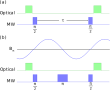
\includegraphics[scale = 0.9]{Ramsey_DC_AC.pdf}  
\caption{\textbf{Pulsed Magnetometry Sequences} \textbf{a)} Ramsey Sequence for DC magnetometry \textbf{b)} Hahn-Echo Sequence for AC magnetometry.}
\label{Fig_two}
\end{figure}

For AC magnetometry, the Ramsey sequence can be modified by bisecting the free precession interval $\tau$ with a single resonant $\pi$ pulse. The pulse is precisely timed to occur at the node of the oscillating field [Fig \ref{Fig_two}(b)] and deems to swap the accumulated phase from the $\ket{1}$ to the $\ket{0}$ state. For slow components of the external magnetic noise, the swap allows the second half of the free precession interval to compensate for phase randomization acquired during the first half of the interval. Using this sequence, $\tau$ can be increased to the homogeneous spin coherence time $T_2$ often orders of magnitude longer than $T_2^*$. The sensitivity for sensing an AC field is then improved when compared to sensing a DC field by a factor $\sqrt{T_2^*/T_2}$. This sequence is known as a Hahn-Echo sequence but AC magnetometry can be performed by more complex dynamical decoupling techniques \cite{carr1954effects, meiboom1958modified}.


\subsection{Rabi oscillations}

When an on- or near-resonant MW pulse is applied to a ground state transition in the NV, e.g. $\ket{0} \rightarrow \ket{+1}$, the NV spin state population will oscillate coherently between these two levels at a rate called the Rabi frequency ($\Omega_R$). This rate of oscillation is a function of the amplitude of the applied MW pulse. It is commonly measured by consecutively applying a polarizing laser pulse, a MW pulse, and a readout pulse [Fig. \ref{Fig1_3} (a)] and varying the MW pulse length after each iteration. 

\begin{figure}[t!]
\centering
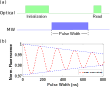
\includegraphics[scale = 0.9]{Rabi_sequence_and_figure.pdf}  
\caption{\textbf{Rabi pulse sequence and oscillations} \textbf{a)} Pulse sequence for detecting Rabi oscillation between two spin sublevels \textbf{b)} Example Rabi oscillations (\textcolor{red}{-- --}) with exponential decay envelope (\textcolor{blue}{ -- --}).}
\label{Fig1_3}
\end{figure}

Fig. \ref{Fig1_3} (b) plots a typical Rabi curve and its decay envelope. If the NV is originally in $\ket{0}$ (ie. at time $t = 0$) and we let the system evolve, then the probability that the spin is found in $\ket{+1}$ is $P_{+1} = \left(\frac{\omega_1}{\Omega_R}\right)^2 sin^2\left(\frac{\Omega_R t}{2}\right)$ where $\Omega_R = \sqrt{(\omega-\omega_0)^2-\omega_1^2}$ is the Rabi frequency, $\omega$ is the radial frequency of the oscillating field $B_1(\omega)$, $\omega_0$ the resonant frequency of the transition, and $\omega_1$ the (max) Rabi frequency at zero detuning. At resonance, the driving frequency is $\omega = \omega_0$ and the transition probability becomes $P_{+1} = sin^2\left(\frac{\omega_1 t}{2}\right)$. In order to therefore drive the entire population from e. g. $\ket{0}$ to $\ket{+1}$ as needed in, for example, the Hahn-Echo sequence described in \ref{Pulsed_Ramsey}, one needs to apply a pulse length such that $sin^2 \left(\frac{\omega_1 t}{2}\right) = 1$ which is satisfied when $t = \frac{pi}{\omega_1}$. For a Ramsey-type sequence that requires an equal superposition between $\ket{0}$ and $\ket{+1}$ one needs to apply half the $\pi$ pulse, $t = \frac{\pi}{2\omega_1}$. The Rabi oscillations however decay due to inhomogeneous broadening of the ensembles linewidth, and are therefore fit by the decaying envelope $\text{exp}\{-\left(PW/T\right)^p\}$, where PW is the pulse width and $T$ and $p$ are fit parameters.

\section{NV-MW coupling}

calculate coupling between NV center and MW photons in cavity.

%% This is an example first chapter.  You should put chapter/appendix that you
%% write into a separate file, and add a line \include{yourfilename} to
%% main.tex, where `yourfilename.tex' is the name of the chapter/appendix file.
%% You can process specific files by typing their names in at the 
%% \files=
%% prompt when you run the file main.tex through LaTeX.

\chapter{The Loop Gap Resonator}

As mentioned in the introduction, for many applied modalities within applications that use NV centers, the MW field (often denoted $B_1$ from NMR nomenclature), requires both high power and high uniformity to achieve high-fidelity quantum-state manipulation over the entire sample volume. As volumes are increased however, to maximize the number of NVs addressed without having a deleterious affect on the optimal measurement time, applying such a field becomes more difficult using standard approaches such as shorted coaxial loops \cite{clevenson2015broadband,chipaux2015magnetic}, microstrip waveguides \cite{andrich2017long,horowitz2012electron}, and 50 $\Omega$-terminated coaxial transmission lines \cite{li2010design,mrozek2015circularly,zhang2016microwave,zhang2018vector}. These broadband approaches allow arbitrary drive frequencies, however, the lack of resonant enhancement forces a compromise between the addressed volume and field strength. Section \ref{Planar} describes how planar lumped-element resonators such as split-ring resonators \cite{bayat2014efficient}, planar-ring resonators \cite{zhang2016microwave,sasaki2016broadband}, omega resonators \cite{twig2013ultra,horsley2018microwave,simpson2017electron}, and patch antennas \cite{zhang2016microwave} can improve coupling between the resonator and the NVs by resonantly enhancing the local $B_1$ field and thus enable MW driving over larger regions, but at the expense of bandwidth and thus, for an operational magnetometer, dynamic range. Additionally, planar resonators are shown to yield poor homogeneity in the planes normal to their surface and therefore lend themselves less to bulk magnetometry than to 2D imaging applications. To address this shortcoming 3D resonators and cavities can be employed such as enclosed metallic cavity resonators \cite{rose2017coherent}, enclosed dielectric resonators \cite{breeze2017continuous,floch2016towards,creedon2015strong}, open dielectric resonators \cite{kapitanova2017dielectric}, and three-dimensional lumped element resonators \cite{angerer2016collective}, which provide good field homogeneity and strong resonantly enhanced fields, but offer little to no optical access. Since all-optical initialization and readout is a primary benefit for many solid-state spin systems, including NV diamond \cite{doherty2013nitrogen}, such a trade-off is incompatible with many existing and envisioned applications \cite{schirhagl2014nitrogen}. 

To address this current shortcoming a three-dimensional tunable loop-gap resonator (LGR), based on the anode block of a cavity magnetron, is used to achieve desired MW drive strengths homogeneously over large areas. Additionally, its open geometry allows for good optical accessibility for interrogation volumes centered within the LGR cavity. Traditionally, the LGR has been used either as the anode block of cavity magnetrons \cite{}, or as a low frequency (2-4 GHz) lumped element resonator for electron paramagnetic resonance (EPR) studies \cite{}.  

\section{Resonant Enhancement of the MW field}

Talk about (with calculations) how Q of the cavity affects field build up in resonator and how resonant enhancement can build strong MW field strengths.

\section{Model}

whatever

\subsection{Lumped element solutions} \label{circuit}

Theoretical framework for analyzing LGR for $m$ loops and $n$ gaps including field distribution calculations

\subsection{Field based solutions}

\subsection{Coupling}

Theory of coupling (mutual inductance, capcitance, etc)

\section{LGR Design}

Due to the loop gap resonator's existence since the early 20th century \cite{collins1948microwave} it has seen many variations and modifications all designed with particular applications in mind. Figure \ref{} shows the cross section of a variety of LGRs including rising-sun, vane, slot, and hole-and-slot type resonators. EPR experiments at low frequencies (2-4 GHz) quickly adopted the LGR as opposed to more traditional TE\textsubscript{102} type cavities because of the LGRs smaller size relative to the frequency of excitation. At 3 GHz the side length of the TE\textsubscript{102} cavity must be at least 5 cm which reduces drastically the cavity filling factor--a parameter necessary for the sensitivity of an EPR signal. Since many aspects of EPR spectroscopy are mirrored in NV magnetometry (requirement of homogeneous and strong microwave signals, frequency of operation, etc.) we selected to design a hole-and-slot type resonator found in many EPR applications \cite{}.  
\vspace{5mm}
\begin{figure}[h!]
\centering
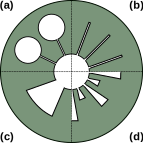
\includegraphics[scale = 0.5]{LGR_Variation.pdf}  
\caption{\textbf{Loop Gap Resonator Variations} \textbf{a)} Hole and Slot. \textbf{b)} Slot. \textbf{c)} Vane. \textbf{d)} Rising Sun - type}
\label{LGR_variation}
\end{figure}


\subsection{LGR}

A standard hole-and-slot LGR with $n$ outer loops can be approximated as $n$ coupled LC resonators oscillating in tandem at a target resonant frequency \cite{wood1984loop}. Circulating currents around the central and outer loops create a total inductance, as found in section \ref{circuit}, 

% When circuit model section is written take out these equations and simply reference them.

\begin{equation}
L \approx \frac{L_c n L_o}{n L_o + L_c},
\end{equation}\label{induct}

and charge at the gap walls create a total capacitance C, which is given by

\begin{equation}
C \approx \frac{\epsilon_r \epsilon_o A}{nd},
\end{equation} \label{cap}

which, when combined yield the resonant frequency

\begin{equation}
f_0 = \frac{1}{2 \pi \sqrt{LC}}.
\end{equation}

\begin{figure}[t!]
\centering
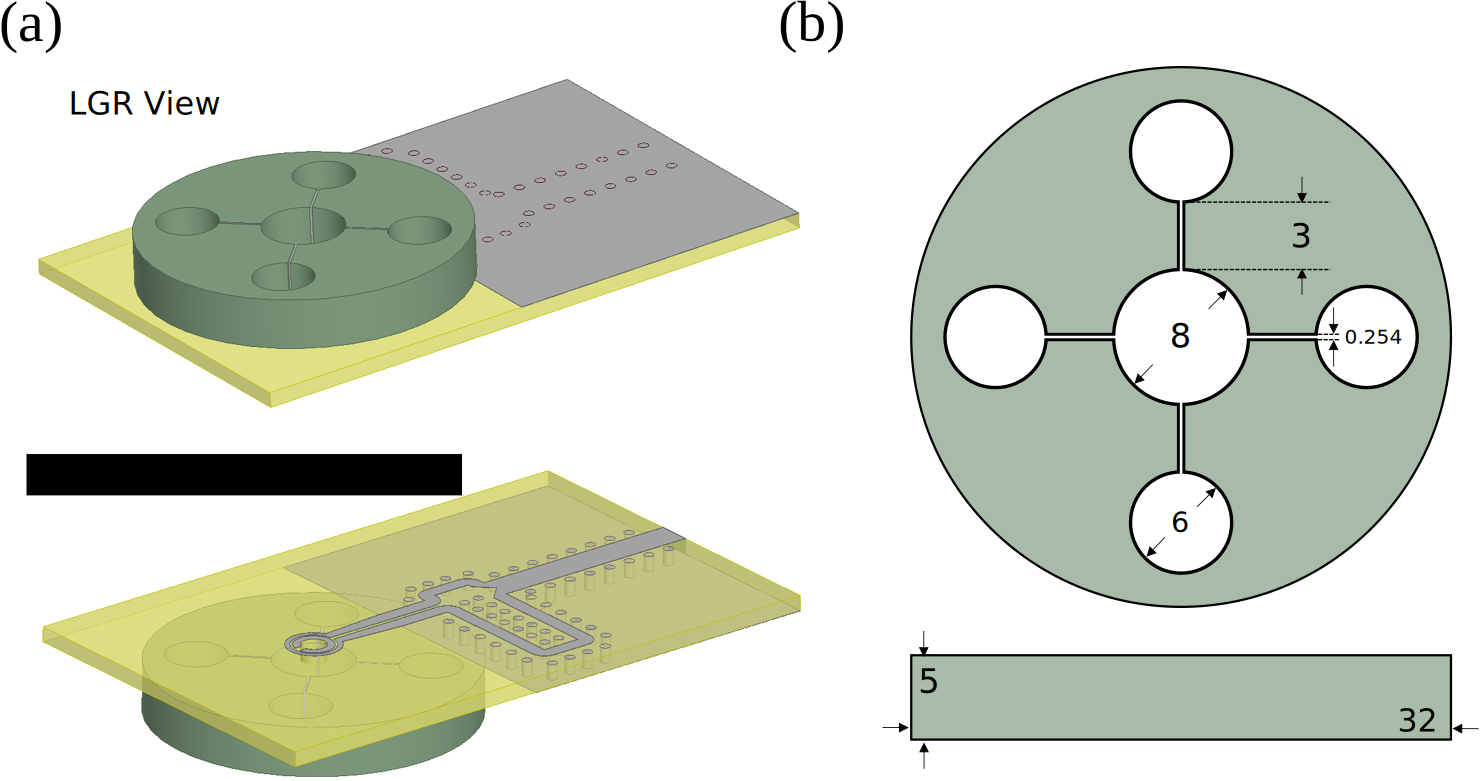
\includegraphics[width = \textwidth]{LGR_Image.pdf}  
\caption{\textbf{Rendering and Wire Diagram of Loop Gap Resonator} \textbf{a)} The metallic resonator employs a five-loop four-gap architecture. Microwaves are coupled into the LGR via the exciter antenna, which is fabricated on a printed circuit board. \textbf{b)} Line drawing of the LGR. All dimensions are in mm. Optional mounting holes and radial access port for laser excitation are now shown.}
\label{LGR_drawing}
\end{figure}

In practice, the central loop diameter is set to $\sim 5-10 $ mm, corresponding to the typical size of a diamond plate. The outer loop diameters are chosen to match the inner diameters within a small factor to ensure return flux is captured and does not extend into the annular region around the LGR \cite{}. Since the outer and inner loops set the effective inductance of the resonator, the gap area $A$ is constrained by the dual LGR design objectives of (i) maintaining optical accessibility, which limits the thickness of the device, and (ii) bounding $f_0$ above the target resonant frequency in order to allow for further tuning vie dielectric shims (discussed in section \ref{tuning}). Additionally, while increasing the number $n$ of loops and gaps can improve $B_1$ uniformity \cite{piasecki1993field} and lower the LGR's resonant frequency, this approach results in a denser mode spectrum \cite{froncisz1982loop} and increases the likelihood of cross-mode excitations deleteriously altering the field distribution within the central loop. As a compromise, the design employs $n=4$ outer loops [Fig. \ref{LGR_drawing} (a)] allowing for sufficient uniformity while locating the closest eigenmode more than 1.5 GHz below the TE\textsubscript{10} eigenmode [Fig \ref{}].  

The LGR in this work therefore consists of a central loop with radius $r_c = 4$ mm surrounded by four symmetrically arranged outer loops of radius $r_o = 3$ mm as shown in Figure \ref{LGR_drawing} (b). The outer loops return magnetic flux to the central loop and therefore oscillate antisymmetrically with the central loop ($\pi$ out of phase). The side walls of the capacitive gaps are separated by $d = 254$ $\upmu$m. With these dimensions, using equations \ref{induct} and \ref{cap}, $L = 8.7$ nH and $C = 0.17$ pF, resulting in an expected resonant frequency for the naked air-gapped LGR of $f_0 = 4.1$ GHz, approximately 1.2 GHz above the NV resonance frequencies.

An eigenfrequency simulation of the resonator using the geometrical parameters listed above was completed in ANSYS HFSS and the distribution of the magnetic flux density ($B_1$) for the TE\textsubscript{10} mode is depicted in Figure \ref{LGR_Eigen}.

\begin{figure}[t!]
\centering
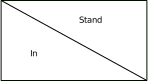
\includegraphics[width = \textwidth]{STANDIN.pdf}  
\caption{\textbf{Eigenfrequency solution to LGR} \textbf{a)} \textcolor{red} {STANDIN. PLEASE REPLACE}}
\label{LGR_Eigen}
\end{figure}








%need to hit on: why 4 loops and 4 gaps, why titanium?

%Eigenfrequency simulations in HFSS for LGR structure. 

%(Real) Mode spectrum 

%etc

%discussion of manufacturing using wire EDM, materials used, milling, etc.

\section{Excitation Design}

Discussion with images of coupling using shorted coax loop.

More robust coupling for implementable device

Discussion of split ring exciter antenna and design outline of feedline and balun and design process of stepping through circuit etc.

center loop coupling with split ring resonator. Sonnet program design or split loop (snap shots from program and S11 etc) 

\section{Tuning} \label{tuning}

Talk about tuning the LGR using sapphire shims; why use sapphirie shims? etc etc etc

\section{Matching}

Talk about matching using coupling parameter and etc. (quick overview of matching using mathematical framework).

Talk about matching using Lateral loop coupling

Talk about Balun design (w/ sonnet)

Talk about board design (w/ sonnet)

Talk about additional matching using stub tuner.




%% This is an example first chapter.  You should put chapter/appendix that you
%% write into a separate file, and add a line \include{yourfilename} to
%% main.tex, where `yourfilename.tex' is the name of the chapter/appendix file.
%% You can process specific files by typing their names in at the 
%% \files=
%% prompt when you run the file main.tex through LaTeX.

\chapter{LGR Performance and Field Characterization} \label{ch3}

In this chapter the LGR electrical and magnetic are discussed and measured. All simulations were completed in ANSYS HFSS a full-wave electromagnetic simulation tool. 

\section{Quality Factor}\label{quality}

As mentioned in section \ref{resonant_enhc}, The quality (or Q) factor of an oscillator quantifies how often (in terms of the oscillation period) the energy will oscillate back and forth until its initial amplitude is reduced by a factor of $1/e$. At critical coupling ($\beta = 1$) the intrinsic Q ($Q_0$) of the resonator (which quantifies the oscillation lifetime due to resistive losses) is calculated as the inverse of its fractional bandwidth ($FBW$),
\begin{equation}
Q_0 = \frac{1}{FBW} = \frac{f_0}{\Delta_{3dB}}.
\end{equation} 
The fractional bandwidth however is calculated from the loaded Q ($Q_L$) which takes into account coupling losses due to power reflection at the exciter antenna/LGR interface. Incorporating these reflections is achieved by assigning an external Q ($Q_e$) to account for these losses. $Q_e$ then combines with $Q_0$ in a parallel configuration
\begin{equation}
\frac{1}{Q_L} = \frac{1}{Q_0} + \frac{1}{Q_e},
\end{equation} 
to yield $Q_L$. The intrinsic Q, $Q_0$, and the external Q, $Q_e$, characterise the most dominant loss mechanisms of the device. Other loss mechanisms and their contribution to $Q_L$ are discussed in reference \cite{piasecki1993field}; they include, but are not limited to, loss in a sample, radiation losses, surface wave losses, hand-shaking (if not properly shielded), etc..

Since the quality factor is inversely proportional to the resonator bandwidth the LGR needs to exhibit fairly low Q in order to address all eight NV resonances and their shifts due to an external field. The LGR was thus designed to accommodate an NV ensemble that has been split using an up-to 14 gauss biasing field $B_0$. Since the NV gyromagnetic ratio ($\gamma_B$) is 2.8 MHz/gauss, this corresponds to an ideal bandwidth of 39 MHz and, at 2.87 GHz, a Q of $\sim$ 36. In addition to a wide dynamic range, a low Q allows for the use of concatenated pulse sequences without employing additional methods to evacuate power from the resonator before the next pulse is applied (e.g. active cancellation). 

\subsection{Ringdown time}\label{ringdown}

As mentioned above, in order to apply concatenated MW pulses to a sample in the LGR (as is done often in NMR and NV applications \cite{}) the power oscillating in the cavity must be evacuated or dissipated in between pulses. One method used is to apply active cancellation techniques that either introduce extra components to the excitation circuitry to abruptly de-tune the resonator before the next pulse is applied  \cite{} or apply a secondary pulse that is designed to destructively interfere with the cavity ring-down \cite{Franck2015Active}. Another, and also the technique applied here, is to make the resonator intrinsically lossy and therefore dissipate the left-over power in the cavity as either heat or radiation. To calculate the ring-down time $\tau_{ring}$ of the LGR we apply a damping exponential to the field within the cavity such that $B(t) = B_{init}e^{-\pi f_0t/Q}$ (neglecting any phase caused by a shift in the resonant frequency), and solving for the time $t$ at which the amplitude has decreased to $1/e \cdot B_{init}$. Doing this yields
\begin{equation}\label{eqn33}
\tau_{ring} = \frac{Q}{\pi f_0}.
\end{equation} 
Using equation \ref{eqn33} and the bandwidth and center frequency extracted from the measured data in Figure \ref{LGR_tuning}, one calculates $\tau_{ring} = 4$ ns which is sufficient for standard NV and NMR pulsed protocols \cite{Smeltzer2009Robust,Jelezko2004Observation,Steiner2010Universal}.

\section{Simulating the Magnetic Field} \label{simField}

The $B_1$ field distribution in the center loop of the LGR was simulated using the full-wave electromagnetics simulation suite ANSYS HFSS. The simulation includes the 200 $\upmu$m dielectric shims and the full exciter circuit depicted in Figures \ref{LGR_Exciter} and \ref{LGR_drawing}. The solution type was set to "driven modal" since the exciter board has a single trace interconnect and thus requires the solution of TE and TM propagation modes. Figure \ref{LGR_simulated} shows the $B_1$ distribution computed by HFSS at an input power of 42 dBm. The exciter board (which extends over the LGR center loop along the line $x = y$ in the figure) clearly imparts a small perturbation on the otherwise radially symmetric field. The simulation predicts $B_1 \approx 4.8$ gauss at the LGR center and a maximum field of $B_1 \approx 5.4$ gauss at the perimeter. Two metrics are used to quantitatively characterize 2D regions of homogeneity , the fractional root-mean-square inhomogeneity $\sigma_{rms}$ calculated as 
\begin{equation}\label{sigma_rms}
\sigma_{rms} = \sqrt{\frac{\Sigma_{i = 1}^N(B_{1,i}-B_{2,i})^2}{N}} \cdot \mu_N^{-1},
\end{equation}
where $i$ is an index over all $B_1$ field values in the region, $N$ is the total number of values, and $\mu_N$ is the mean of all $N$ values, and the fractional peak-to-peak variation $\sigma_{pp}$ calculated as
\begin{equation}\label{sigma_pp}
\sigma_{pp} = \frac{\left[B_1^{max} - B_1^{min}\right]}{\mu_N}.
\end{equation} 
The use of both metrics facilitates comparison with alternative existing designs. Within a 32 mm\textsuperscript{2} circular area centered in the LGR central loop, simulations indicate $\sigma_{rms} = 3.8\%$ and $\sigma_{pp} = 11\%$, whereas in a smaller 11 mm\textsuperscript{2} circular area, simulations indicate $\sigma_{rms} = 1\%$ and $\sigma_{pp} = 2\%$.

\begin{figure}[t!]
\centering
\includegraphics[scale = 0.75]{FieldSimulation.pdf}  
\caption{\textbf{Simulated magnetic field} Top-down cross section of center loop of LGR. Slice is taken at half height h. Simulations suggest the $B_1$ field distribution
should be approximately radially symmetric, with the leading order deviation resulting from the exciter antenna. Dashed lines indicate the 32 mm\textsuperscript{2} and 11mm\textsuperscript{2} areas within which the $B_1$ field uniformity is evaluated.}
\label{LGR_simulated}
\end{figure}

As a three dimensional cavity resonator, the LGR provides better axial field uniformity than planar-only geometries \cite{floch2016towards,kapitanova2017dielectric,angerer2016collective}. Figure \ref{LGR_axial_simulated} plots the simulated $B_1$ along the LGR's symmetry axis, illustrating the improved axial field uniformity possible with three-dimensional cavity
resonators, compared to that of planar-only geometries. The presence of the split ring resonator at $z = 4.024$ mm perturbs $B_1$ inside the LGR, shifting the point of maximal $B_1$ down by 0.4 mm, away from the split-ring resonator. Within a cylindrical volume of 3.14 mm\textsuperscript{3} (1 mm radius and 1 mm thickness), centered around the point of maximal $B_1$, the simulations predicts $\sigma_{rms} = 0.78\%$ and $\sigma_{pp} = 3.7\%$. For a larger cylindrical volume of 12.6 mm\textsuperscript{3} (2 mm radius and 1 mm thickness), the simulation predicts $\sigma_{rms} = 2\%$ and $\sigma_{pp} = 8\%$. These dimensions are comparable to those of commercially available single-crystal diamonds. Additionally, Figure \ref{LGR_axial_simulated} gives 1D regions of homogeneity along the LGR symmetry axis.

\begin{figure}[t!]
\centering
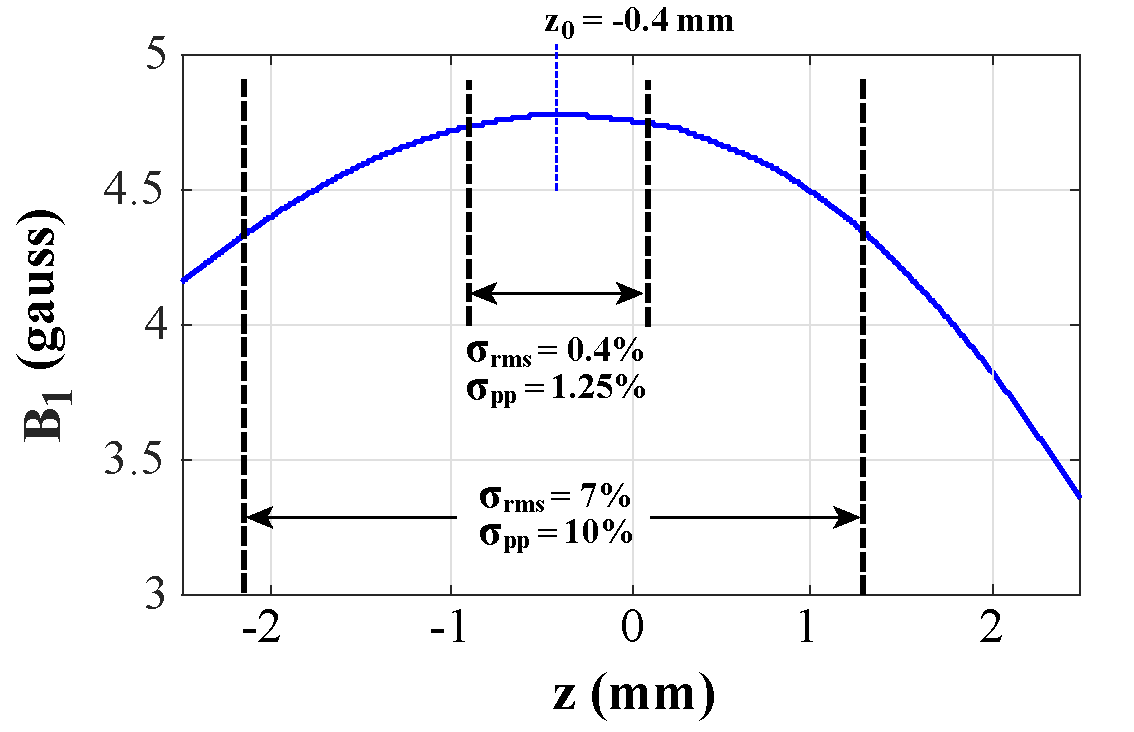
\includegraphics[scale = 0.7]{Figure_B_2.pdf}  
\caption{\textbf{Simulated $B_1$ field along LGR symmetry axis.} The symmetry plane of the LGR is located at $z = 0$ mm. The edges of the LGR are at $z = \pm 2.5$ mm, and the split-ring resonator is located at $z = 4.024$ mm. The presence of the split-ring resonator shifts the point of maximal $B_1$ off-center to $z_0 = -0.4$ mm.}
\label{LGR_axial_simulated}
\end{figure}

\section{Measuring the Magnetic Field} \label{field}

Measuring the magnetic field distribution within the central loop of the LGR can be done in several ways. The simplest is to raster scan a magnetic probe across the cross section one wants to measure. However there are many drawbacks to this method. First, the spatial resolution is set by the size of the probe tip. Figure \ref{LGR_probe} shows the normalized magnetic field distribution of the LGR, measured by a 100B Beehive magnetic probe. The shielded loop diameter of the probe is 1 mm and thus the resolution is poor. Second, the probe has very little access to the center of the cavity. The data in Figure \ref{LGR_probe} was, for example, taken 1 mm above the LGR center loop; a region in which the magnetic field is highly divergent. Since the magnetic loop only measures the component of the field that lies parallel with its cental axis this provides a limited picture of the total field distribution. Third and finally, the proximity of the probe to the LGR perturbs the field and thus the distribution measured is an altered version of the unperturbed scenario. 

Another method--with similar drawbacks--is to measure the cavity transmission characteristics under intentional perturbation by a metal probe tip. by moving the perturbing probe tip, the transmission parameter $S_{21}$ (when an out-coupler loop is placed into one of the lateral loops) changes proportional to the field at the point of measurement. Thus, if the metal tip is scanned across the cavity, a picture of the field distribution can be extracted.  

\textcolor{red}{Since the LGR in this thesis is designed to supply MWs to NV centers, one can utilize the NV centers in turn to measure the strength of the supplied MWs}. If the period of the Rabi frequency (as described in section \ref{Rabi}) can be determined, then one can, using a simple relation, calculate the magnitude of $B_1$. This measurement of the field does not suffer from the drawbacks of the other two mentioned above and thus, it's the method employed in this thesis. The following subsections describe the measurement apparatus, measurement process, and calculations used to infer the strength of the $B_1$ field at various points within the LGR center loop.

\begin{figure}[t!]
\centering
\includegraphics[width = \textwidth]{probefield.pdf}  
\caption{\textbf{$B_z$ component of field measured with probe} \textbf{a)} 3D surface plot of $B_z$ field distribution using a Beehive 100B magnetic field probe. Color bar units are normalized magnetic field. Normalized to their maximum value. \textbf{b)} Same data as in a) but top-down view. }
\label{LGR_probe}
\end{figure}

\begin{landscape}
\begin{figure}[b!]
\centering
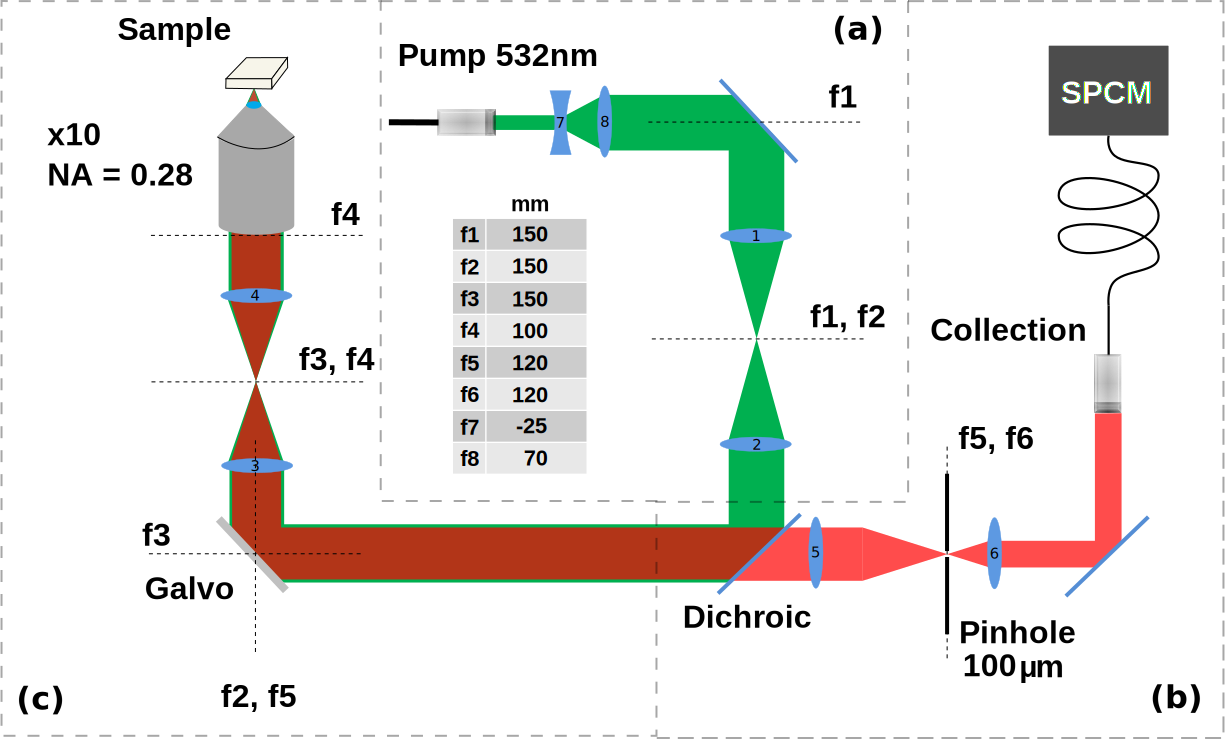
\includegraphics[scale = 0.7]{Confocal_Diagram_001.pdf}  
\caption{\textbf{Confocal Microscope} Custom built confocal microscope used to measure $B_1$ in LGR.}
\label{LGR_confocal_diagram}
\end{figure}
\end{landscape}

\subsection{Experimental setup} \label{setup}

To measure the field distribution within the LGR center loop a home-built scanning confocal microscope [Figure \ref{LGR_confocal_image}] was employed. The confocal microscope supplies the 532 nm pump beam to polarize the NVs and collects the resulting fluorescence using a dichroic beam splitter and a single photon counting module (SPCM). The three main sections of the experimental setup are the pump path, the collection path, and the sample path. The pump path [Figure \ref{LGR_confocal_diagram} (a)] includes all optics from the launch of the excitation beam to the dichroic. Optical pulsing is accomplished using an acousto-optic modulator (AOM) that is located before the fiber launch; Ie. the laser passes through an AOM and is then coupled into a single mode (SM) polarization maintaining fiber which is then launched as the pump beam. The SM fiber picks off the first order refracted beam of the AOM and rejects the rest so no iris needed. The pump path contains a fiber launch (FiberPort coupler PAF-X-11-B), a half wave plate to selectively excite and address NV orientations, a beam expander consisting of a positive and negative focal length lens, and a 1:1 telescope. The 1:1 telescope (ie. no magnification) serves to change the angle of the beam down the sample path without moving the excitation spot off the galvo mirrors. In order for this to happen, the distance between the center of the two galvo mirrors and the last lens of the telescope must be equal to the focal length of the lens. In this way the angle of the beam into the objective can be changed without needing to reposition the galvos---which is a function designed for convenience only. The beam expander changes the collimation of 532 nm into the objective and therefore changes where the green comes into focus along the optical axis of the objective. This effectively serves to overlap the green excitation and the red fluorescence. Overlapping the two beams serves to maximize collection through the pinhole on the collection arm since the pinhole is initially aligned using the back-reflected green pump laser.

\begin{figure}[t!]
\centering
\includegraphics[scale = 0.35]{DSC05087.jpg}  
\caption{\textbf{Image of Scanning Confocal Microscope} Custom built scanning confocal microscope used to measure the $B_1$ distribution in the LGR}
\label{LGR_confocal_image}
\end{figure}

The collection path (or arm) [Figure \ref{LGR_confocal_diagram} (b)] begins at the dichroic and ends at the collection end through a multimode fiber (65 $\upmu$m core) and into the SPCM. The path consists of the dichroic, a pinhole between two telescoping lenses, a multimode fiber, and an SPCM. The dichroic (Semrock Brightline FF552-Di02-25x36) filters the green pump beam from the sample fluorescence by reflecting wavelengths below 552nm and transmitting everything above. The first lens of the telescope focuses the beam down and passes it through a pinhole that spatially filters the image in X and Y to provide improved resolution. The pinhole was chosen to be 100 $\upmu$m to maximize collection while sacrificing some lateral resolution in the image. Generally the pinhole diameter ($p_d$) should be selected using the following equation:
\begin{equation}
p_d = \frac{1.22 \lambda}{NA} \cdot M_{objective} \cdot M_{telescope} 
\end{equation}
The telescope in the sample path de-magnifies the beam by a factor $M_{telescope} = \frac{100}{150} = 0.67$ which is the ratio of the focal lengths of the lenses in the sample path. The objective used has a magnification of x10 which leads to a nominal pinhole size of 20 $\upmu$m. However, this limits the amount of fluorescence collected because the pinhole filters out-of-focal-plane light which constitutes a large part of the signal. Since measuring the $B_1$ field distribution in the LGR center cavity does not require high spatial resolution, a 100 $\upmu$m diameter pinhole was chosen such that each measurement wasn't fluorescence starved. The filtered beam then passes through a second lens which focuses it onto the core of a multimode fiber connected to the SPCM. The multimode fiber allows for some rejection of ambient light without too much loss of the fluorescence signal. To further minimize the collection of ambient light, the multimode fiber dock and SPCM are enclosed in a light tight box. 

The sample path [Figure \ref{LGR_confocal_diagram} (c)] also begins at the dichroic, but passes through the galvanometer and objective and ends at the sample within the LGR center loop. It consists of a galvanometer, a 4F lens system (telescope), an iris, an objective and a sample stage. The objective used (Mitutoyo 378-803-3, M Plan Apo 10x $NA=0.28$) has a long working distance of 34 mm. The long working distance was necessary to minimize perturbations of the $B_1$ field by the metal housing of the objective. Future NV wide-field imaging applications may require ceramic-tipped objectives. Finally, although this microscope has a galvanometer capable of scanning the beam over an area of $\sim$ 250 $\upmu$m x 250 $\upmu$m the beam was held steady and the resonator moved to ensure $B_0$ is consistent for all measurements across the central loop of the LGR.


\subsection{Measurement process} \label{measurement}

\begin{figure}[t!]
\centering
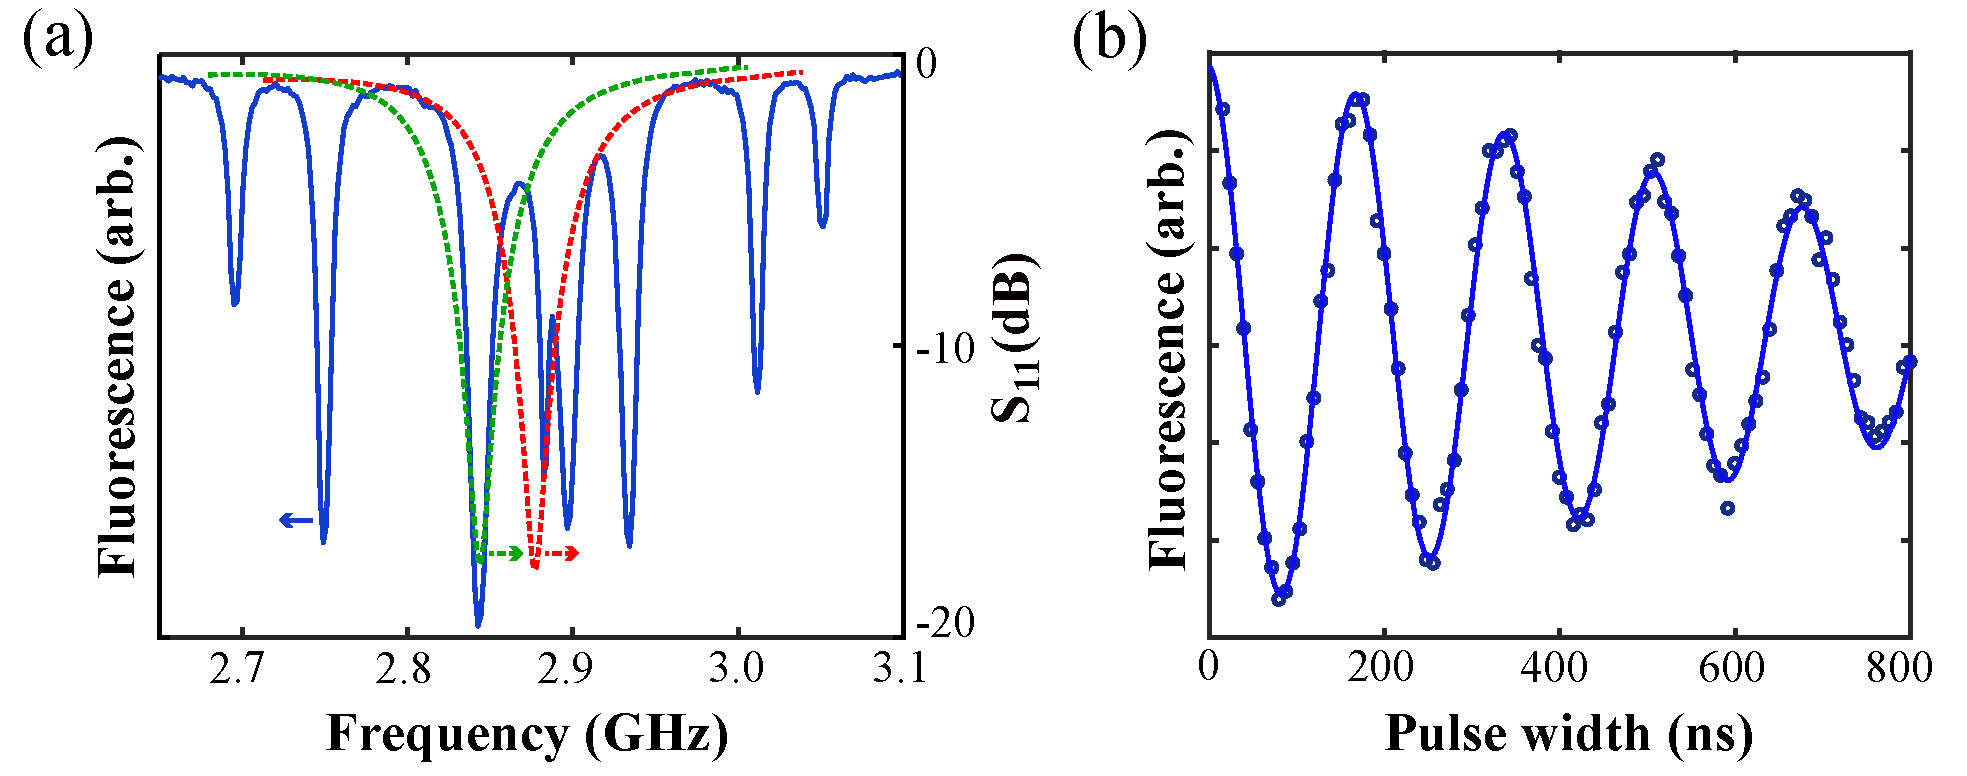
\includegraphics[scale = 0.45]{Figure_3.pdf}  
\caption{\textbf{LGR driving of an NV ensemble} \textbf{(a)} NV electron spin resonance spectrum (\textcolor{blue}{\textbf{---}}) under application of bias field $B_0$. The bias field allows individual addressing of all eight NV resonances, arising from the combination of the two allowed magnetic dipole transitions with the four possible NV orientations. The NV hyperfine structure is obscured by MW power broadening and the contrast variation between the NV resonances is attributed primarily to the $S_{11}$ line-shape. The $S_{11}$ parameter is shown before (\textcolor{red}{\textbf{-\,-\,-}}) and after (\textcolor{dolla-bill}{\textbf{-\,-\,-}}) shifting the LGR resonant frequency $f_0$ to the target NV resonance. Arrows indicate corresponding y axes. \textbf{(b)} Typical data depicting Rabi oscillations under MW excitation at the target NV resonance frequency indicated in (a). Data (\textcolor{navyblue}{$\mathbf{\circ}$}) is fit (\textcolor{blue}{\textbf{---}}) to an exponentially decaying sinusoid.}
\label{LGR_Rabi_meas}
\end{figure}

The strength and homogeneity of $B_1$ within the LGR central loop is evaluated employing standard NV techniques, as described in detail if references \cite{pham2013magnetic,childressthesis2011coherent,mazethesis2010quantum}. More specifically, a custom built scanning confocal microscope (as described in section \ref{setup}) measures the Rabi nutation frequency $\Omega_R$ of an ensemble of NV centers. A $\{$100$\}$-cut diamond plate containing $\sim 1 \times 10^{14}$ NV/cm$^3$ is mounted at the center of the LGR with the $<$100$>$ crystallographic axis collinear with the LGR axis. A rare earth magnet creates a static magnetic bias field $B_0$, which shifts the energies of the $m_s=\pm1$ ground-state Zeeman sublevels. The energy shifts are given to first order by~\cite{taylor2008high}
\begin{equation}
\Delta E \approx \text{g}_{\text{s}} \upmu_\text{B} m_s \vec{B}_0\cdot \hat{n}_i,
\end{equation}
where $\hat{n}_i$ denotes a unit vector oriented along one of the four diamond crystallographic axes. By judicious choice of $\vec{B}_0$, all eight energy levels and associated $m_s\!=\!0\! \leftrightarrow \!m_s\! =\!\pm1$ magnetic dipole transitions can be isolated as shown in Fig. \ref{LGR_Rabi_meas}(a). The resonator is tuned to excite a single NV transition, yielding Rabi oscillations [Fig. \ref{LGR_Rabi_meas}(b)]. The data is fit to an exponentially decaying sinusoid in order to extract the Rabi frequency $\Omega_R$, from which the magnitude of $B_1$ can be calculated as
\begin{equation}\label{B1fromRabi}
B_1 = \sqrt{3}\frac{\hbar \Omega_R}{\text{g}_{\text{s}} \upmu_{B}}.
\end{equation} 
In this geometry, the $B_1$ field is oriented along the [100] crystallographic axis of the diamond, degenerately offset from all four NV axis orientations by half the tetrahedral bond angle $\theta_{\text{tet}}/2 = \text{ArcCos}\frac{1}{\sqrt{3}} \approx 54^\circ$. NV Rabi oscillations are driven by the $B_1$ field component transverse to the NV symmetry axis, reducing the Rabi frequency by $\sqrt{2/3}$ \cite{sasaki2016broadband}. Accounting for the rotating wave approximation introduces another factor of $1/\sqrt{2}$ resulting in the conversion factor $\sqrt{3}$ in equation \ref{B1fromRabi}. To ensure $\vec{B}_0$ is consistent for all measurements across the LGR central loop, the confocal excitation volume is held fixed with respect to the $B_0$-generating permanent magnet, and the diamond and LGR composite device are translated together. The process is then repeated at a locus of points within the LGR center loop (discussed below in section \ref{LGRfield}).

%A static magnetic field ($B_0$) is applied to split the NV resonances and the sapphire shims (tuning process described in section \ref{tuning} are adjusted to tune the resonator to a single NV resonance as shown in Figure \ref{LGR_Rabi_meas} (a). A long working distance objective collects the NV fluorescence while its 34 mm working distance mitigates the effect of the metal objective housing on $B_1$. To measure $\Omega_R$ the NVs within the confocal volume are consecutively polarized, driven, and read out while sweeping the pulse length of the MW driving field. Using a gated single photon counting module, the fluorescence is collected and plotted against the MW pulse length

% Talk about experiment taking Rabi data, ie. Rabi pulse sequence, moving resonator, checking ESR, choosing ESR etc.

%\subsection{$B_1$ from Rabi} \label{calcRabi}
%
%calculating $B_1$ from Rabi frequency using rotating wave approx. etc, essentially where sqrt(3) comes from.


\begin{figure}[t!]
\centering
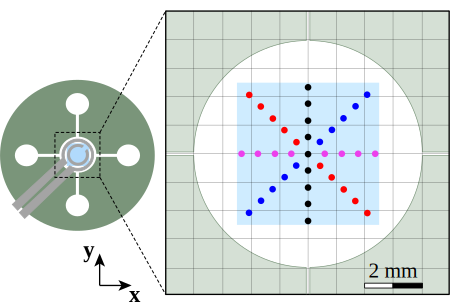
\includegraphics[scale = 1]{Locus_Points.pdf}  
\caption{\textbf{Locus of Measurement Points}  An NV-containing 4.5 mm $\times$ 4.5 mm diamond plate is placed in the LGR central loop, and the  Rabi frequency is measured where indicated (\textcolor{deepmagenta}{\textbullet},\textcolor{black}{\textbullet},\textcolor{red}{\textbullet},\textcolor{blue}{\textbullet}) to characterize $B_1$.}
\label{LGR_Locus}
\end{figure}


\section{LGR field distribution} \label{LGRfield}

The measurement described above is applied at a locus of points in the center of the LGR [Figure \ref{LGR_Locus}]. Since the field distribution is radially symmetric the rest of the field values can be determined from the provided measurements. Application of incident MW power $P \approx 42$ dBm yields an axially oriented $B_1$ at the center of the LGR with magnitude 4.7 G. The corresponding Rabi frequency $\Omega_R = 2\pi \times 7.7$ MHz for NV centers oriented at half the tetrahedral bond angle relative to the LGR axis. Qualitatively, as shown in Figure \ref{LGR_Field_Image} $B_1$ (calculated using equation \ref{B1fromRabi})displays a minimum at the LGR center, increases in magnitude with increasing radial displacement from the center, and is approximately radially symmetric. The best homogeneity is therefore expected at the LGR center. Using equations \ref{sigma_rms} and \ref{sigma_pp} we calculate that, over a 32 mm\textsuperscript{2} circular area axially centered in the LGR
central loop, we observe $\sigma_{rms} = 3.2\%$ and $\sigma_{pp} = 10.5\%$, as shown in Figure \ref{LGR_Field_Image}. Over a smaller 11 mm\textsuperscript{2} circular area, a $\sigma_{rms} = 1.6\%$ and $\sigma_{pp} = 3\%$ is observed. Additionally, as a three-dimensional cavity resonator, the LGR provides better axial field uniformity than planar-only geometries \cite{floch2016towards,kapitanova2017dielectric,angerer2016collective}. For example, for a 3.14 mm\textsuperscript{3} cylindrical volume (1 mm radius disk with 1 mm thickness), simulations yield $\sigma_{\text{rms}}=0.8\%$, $\sigma_{\text{pp}}=3.7\%$ and an average $B_1$ of 4.8 G (see section \ref{simField}).


\begin{figure}[t!]
\centering
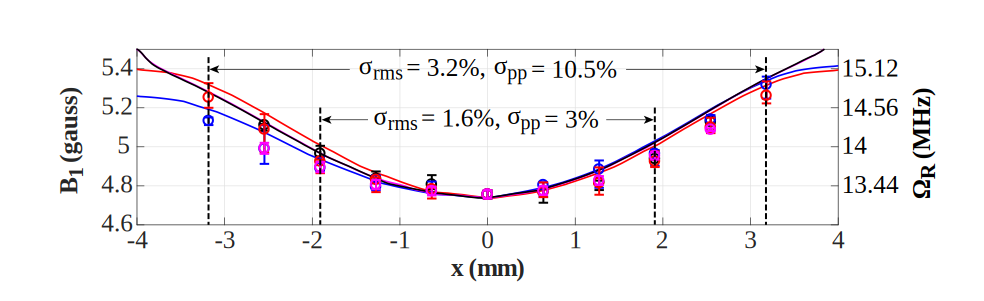
\includegraphics[scale = 0.7]{B1Field.pdf}  
\caption{\textbf{$\boldsymbol{B_1}$ field uniformity of LGR composite device.} $B_1$ field measurements (\textcolor{deepmagenta}{$\circ$},\textcolor{black}{$\circ$},\textcolor{red}{$\circ$},\textcolor{blue}{$\circ$}) at the points depicted in \ref{LGR_Locus} and simulations (\textcolor{deepmagenta}{\textbf{--}},\textcolor{black}{\textbf{--}},\textcolor{red}{\textbf{--}},\textcolor{blue}{\textbf{--}}) along each locus of points are in good agreement. Error bars indicate 1-sigma uncertainty for the $B_1$ measurement. Dashed lines indicate the radial boundaries of the 32 mm$^2$ and 11 mm$^2$ areas over which $B_1$ field uniformity is evaluated. The measured $B_1$ uniformity is given for each area.}
\label{LGR_Field_Image}
\end{figure}




%% This is an example first chapter.  You should put chapter/appendix that you
%% write into a separate file, and add a line \include{yourfilename} to
%% main.tex, where `yourfilename.tex' is the name of the chapter/appendix file.
%% You can process specific files by typing their names in at the 
%% \files=
%% prompt when you run the file main.tex through LaTeX.

\chapter{Discussion and Outlook} \label{ch4}

The device presented here exhibits further benefits along with extensions tailored for specific applications. For example, for ubiquitously employed pulsed measurement protocols, a short ring-down time $\tau_\text{ring}$ (i.e., $B_1$ field $1/e$ decay time) is necessary for high-fidelity pulse shape control. Although techniques to compensate for long ring-down times are effective~\cite{tabuchi2010total,borneman2012bandwidth,peshkovsky2005rf}, shorter native values of $\tau_\text{ring}$ are nonetheless generally desired~\cite{pfenninger1995general,rinard2005loopgap}. The observed loaded quality factor $Q_L = 36$ corresponds to a ring-down time of $\tau_\text{ring} = 4$ ns (see section \ref{ringdown}), making the device suitable for standard pulsed protocols~\cite{Smeltzer2009Quantum, Jelezko2004Observation}. Additionally, a device manufactured with a smaller central loop featured in the appendix section \ref{smallLGR} achieves $Q_L =25.4$ corresponding to a $\tau_{ring}$ of 2.8 ns.

%This ring-down time is expected to allow pulsed MW protocols for high fidelity manipulation of the NV quantum state without deleterious ring-down artifacts.

Due to the square-root scaling of $B_1$ with an incident MW power ($B_1 \propto \sqrt{P}$, see equation \ref{B1approx}), higher power handling can allow for stronger $B_1$ fields. The non-planar resonator design allows for otherwise higher incident MW powers as currents circulate over an extended 2D surface (versus the 1D edge for a planar structure). Furthermore, the metallic LGR thermal mass and  thermal conductivity allow for efficient heat transfer and sinking, which results in improved device stability and power handling. Although the latter was not tested, the LGR composite device is expected to allow $>\!$ 100 W for CW and pulsed operation, limited by the dielectric breakdown of air in the 260 $\upmu$m capacitive gaps. Should available MW power be constrained, stronger $B_1$ strengths can be achieved by fabricating the LGR from a more electrically conductive material (e.g. silver or copper) at the expense of bandwidth (see section \ref{CopperLGR}). In such circumstances, the bandwidth can be continuously adjusted above its minimum value by over-coupling the resonator (at the expense of reduced $Q_L$). 

While the presented LGR is 5 mm thick, the fundamental hole-and-slot approach is expected to be feasible for a variety of thicknesses. A thicker device will provide better field uniformity at the expense of optical access. In contrast, for applications requiring MW delivery over a thin planar volume, the LGR can be fabricated via deposition on an appropriate insulating substrate, as discussed in Refs.~\cite{twig2013ultra,twig2010sensitive}. Semi-insulating silicon carbide~\cite{schloss2018simultaneous} is a suitable substrate due to the material's high thermal conductivity ($\approx$490 W/(m*K)~\cite{protik2017phonon,qian2017anisotropic}, high Young's modulus, moderate cost and wide availability in semi-conductor grade wafers. Further simulations suggest the planar LGR approach can offer modest improvements in $B_1$ homogeneity over split-ring resonators. 

Although the exciter antenna (see Section \ref{excitation}) facilitates a compact, vibration-resistant, and portable device, this component introduces non-idealities in both the field uniformity and optical access. As similar scattering parameters are obtained by inductively coupling a small coil to one of the LGR outer loops, this latter solution may find favor for applications requiring maximal optical access and, furthermore, requires no PCB fabrication.

In this work, a broadband tunable LGR allowing appplication of strong homogeneous MW fields to an NV ensemble was presented and discussed. The LGR demonstrates a dramatic improvement over prior MW delivery mechanisms, both improving on and spatially extending MW field homogeneities. We expect the device to be useful for bulk sensing~\cite{acosta2009diamonds,wolf2015subpicotesla,clevenson2015broadband,chatzidrosos2017miniature,barry2016optical} and particularly imaging applications~\cite{karaveli2016modulation,glenn2015single,barry2016optical,lesage2013optical,wu2016diamond,fu2014solar,glenn2017micrometer}, due to the optical access allowed by the LGR composite device both above and below the diamond.





\appendix
\chapter{LGR variations} %This title needs fixing

\section{Smaller Cavity LGR} \label{smallLGR}
\begin{figure}[b!]
\centering
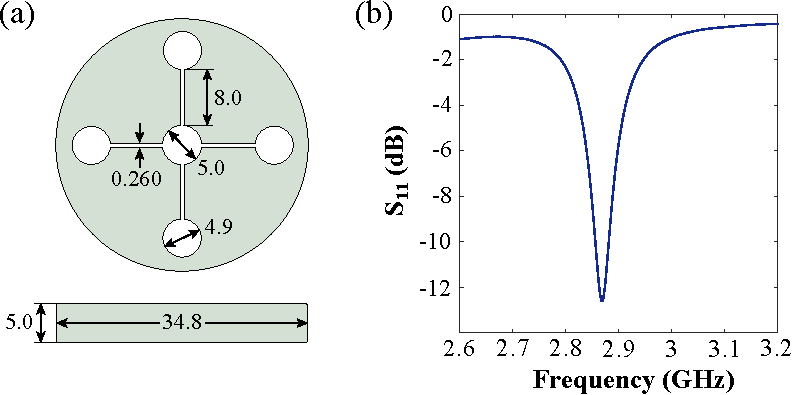
\includegraphics[width = \textwidth]{Figure_B_3.pdf}  
\caption{\textbf{Smaller LGR design} \textbf{(a)} Line drawing of smaller LGR with central loop radius $r_c = 2.5$ mm as described in section \ref{smallLGR}. Units are in mm. \textbf{(b)} Measured $S_{11}$ for composite device tuned to $f_0 \approx 2.87 GHz$.}
\label{smallLGRfigure}
\end{figure}   
To achieve stronger MW driving, we also designed and fabricated
smaller LGR with central loop radius $r_c = 2.5$ mm and $n = 4$ outer loops of radius $r_o = 2.45$ mm, as shown in Figure \ref{smallLGRfigure}. The naked air-gapped LGR cavity exhibits $f_0 = 4.5$ GHz, similar to the larger LGR design described in the main text. Employing the same exciter antenna, $B_1 = 5.8$ gauss is measured at the center of the smaller LGR device. The measured 3 dB bandwidth $\Delta_{3dB} = 112$ MHz corresponds to a loaded quality factor of $Q_L = 25.4$, and an associated ring-down time of 2.8 ns.


\begin{figure}[t!]
\centering
\includegraphics[width = \textwidth]{CopperLGR.pdf}  
\caption{\textbf{Copper Loop Gap Resonator} Loop Gap Resonator manufactured from C145 machinable copper}
\label{LGR_Copper}
\end{figure}   


\section{Copper LGR} \label{CopperLGR}

To achieve higher Q-factors without redesigning the LGR geometry one can fabricate the device from a more conductive material such as copper ($\sigma_c = 59 \times 10^6$ S/m). We manufactured an LGR in C145 machinable copper [Figure \ref{LGR_Copper}]. Figure \ref{LGR_Coppervstit} plots the reflection coefficient $S_{11}$ of both the copper and titanium LGR. Both are critically coupled and the Q factor (for the copper LGR) is measured to be 287, a $>\times 10$ improvement over the titanium device. Such an LGR can be desirable when bandwidth is not a limiting factor and stronger fields are required. The copper LGR has the same dimensions as the smaller cavity LGR in section \ref{smallLGR} that exhibits a Q of 25.4. Re-scaling the measured $B_1$ in the LGR center by $\sqrt{287}/\sqrt{25.4}$ yields the theoretical field strength in the center of the copper resonator. In this case the copper resonator is predicted to have a $B_1$ field strength of $\sim 19.5$ gauss in the center of the center loop.  

\begin{figure}[t!]
\centering
\includegraphics[scale = 0.85]{copperVStitanium.pdf}  
\caption{\textbf{Copper vs. Titanium LGR} Scattering parameters ($S_{11}$) of the copper manufactured LGR (\textcolor{blue}{---}) in comparison to titanium LGR (\textcolor{red}{---})}
\label{LGR_Coppervstit}
\end{figure} 

\section{Shielding}  

Fields that extended away from the LGR (ie. fields that aren't fully caught by the flux return loops) as well as fringing fields above and below the resonator can lead to handshaking or radiation losses if the resonator is not properly shielded during operation. However, because shielding limits the optical accessibility of the center loop and because bandwidth optimization is not the primary concern for the LGR's use as a MW drive source for NVs, shielding was not addressed during the experiment outlined in section \ref{measurement}. For the sake of completeness however, it should be mentioned that proper lateral shielding of the LGR can increase Q factors by minimizing the aforementioned loss mechanisms \cite{petryakov2001bridged, rinard2005loopgap}. Using a copper tube approximately $\times 1.5$ the full diameter of the LGR, an almost doubling of the LGR Q factor (from 287 to $\sim 470$) was achieved. Applying the same calculation as above, a $B_1$ field strength of $\sim 25$ gauss is expected when the copper resonator is properly shielded.   

\clearpage
\newpage

%\include{appb}
\include{biblio}
\end{document}

